
%%%%%%%%%%%%%%%%%%%%%%%%%%%%%%%%%%%%%%%%%%%%%%%%%%%%%%%%%%%%%%%%%%%%%%%%%%%%%%%%
% This LaTeX document is a comprehensive study guide for a chemistry exam.
% It is structured to provide a clear, phased study plan and detailed explanations
% of practice problems relevant to the exam topics.
%
% Preamble: Loading necessary packages for formatting and functionality.
%%%%%%%%%%%%%%%%%%%%%%%%%%%%%%%%%%%%%%%%%%%%%%%%%%%%%%%%%%%%%%%%%%%%%%%%%%%%%%%%
\documentclass{article}

% PACKAGES ---------------------------------------------------------------------
% The 'geometry' package allows for easy customization of page dimensions.
\usepackage[letterpaper, margin=1in, textwidth=6.5in]{geometry}
% The 'graphicx' package is used for including images.
\usepackage{graphicx}
% The 'amsmath', 'amssymb', and 'amsfonts' packages provide advanced mathematical typesetting.
\usepackage{amsmath}
\usepackage{amssymb}
\usepackage{amsfonts}
% The 'enumitem' package allows for customization of list environments.
\usepackage{enumitem}
% The 'pdfpages' package is used to include external PDF documents.
\usepackage{pdfpages}
% The 'mhchem' package is used for typesetting chemical formulas and equations easily.
\usepackage[version=4]{mhchem}

% DOCUMENT START ---------------------------------------------------------------
\begin{document}

% TITLE ------------------------------------------------------------------------
% Creates a title for the study guide.
\title{\textbf{Comprehensive Study Guide for Chemistry Exam 2 \\ Chapters 5, 8, \& 9}}
\date{} % No date is displayed
\maketitle

%%%%%%%%%%%%%%%%%%%%%%%%%%%%%%%%%%%%%%%%%%%%%%%%%%%%%%%%%%%%%%%%%%%%%%%%%%%%%%%%
% CHAPTER 5: Ionic and Covalent Compounds
%%%%%%%%%%%%%%%%%%%%%%%%%%%%%%%%%%%%%%%%%%%%%%%%%%%%%%%%%%%%%%%%%%%%%%%%%%%%%%%%
\subsection*{Chapter 5: Ionic and Covalent Compounds}

\subsubsection*{1. Classifying Ionic vs. Molecular Compounds}
\begin{itemize}[itemsep=5pt]
    \item \textbf{Ionic Compounds} are formed between a \textbf{metal} (cation) and a \textbf{nonmetal} (anion). Electrons are transferred from the metal to the nonmetal, creating charged ions that are held together by electrostatic attraction. For example, NaCl is formed from the metal Na and the nonmetal Cl.
    \item \textbf{Molecular (Covalent) Compounds} are formed between two or more \textbf{nonmetals}. Electrons are shared between atoms to form covalent bonds. For example, \ce{H2O} is formed from the nonmetals H and O.
\end{itemize}

\textbf{Practice Problems:} Classify each of the following as ionic or molecular.
\begin{enumerate}[itemsep=5pt]
    \item \textbf{Ionic Examples:}
    \begin{enumerate}
        \item \ce{FeCl3}: Iron (Fe) is a metal, Chlorine (Cl) is a nonmetal. $\rightarrow$ \textbf{Ionic}
        \item \ce{K2O}: Potassium (K) is a metal, Oxygen (O) is a nonmetal. $\rightarrow$ \textbf{Ionic}
        \item \ce{Mg3(PO4)2}: Magnesium (Mg) is a metal, and phosphate (\ce{PO4^3-}) is a polyatomic anion (composed of nonmetals). The bond between Mg and the phosphate group is ionic. $\rightarrow$ \textbf{Ionic}
        \item \ce{Ca(OH)2}: Calcium (Ca) is a metal, and hydroxide (\ce{OH-}) is a polyatomic anion. The bond between Ca and the hydroxide group is ionic. $\rightarrow$ \textbf{Ionic}
        \item \ce{AlP}: Aluminum (Al) is a metal, Phosphorus (P) is a nonmetal. $\rightarrow$ \textbf{Ionic}
    \end{enumerate}
    \item \textbf{Molecular Examples:}
    \begin{enumerate}
        \item \ce{SO2}: Sulfur (S) and Oxygen (O) are both nonmetals. $\rightarrow$ \textbf{Molecular}
        \item \ce{N2O4}: Nitrogen (N) and Oxygen (O) are both nonmetals. $\rightarrow$ \textbf{Molecular}
        \item \ce{PCl5}: Phosphorus (P) and Chlorine (Cl) are both nonmetals. $\rightarrow$ \textbf{Molecular}
        \item \ce{CH4}: Carbon (C) and Hydrogen (H) are both nonmetals. $\rightarrow$ \textbf{Molecular}
        \item \ce{SiCl4}: Silicon (Si) is a metalloid that bonds covalently with nonmetals like Chlorine (Cl). $\rightarrow$ \textbf{Molecular}
    \end{enumerate}
\end{enumerate}

\bigskip
\subsubsection*{2. Lattice Energy}
\begin{itemize}[itemsep=5pt]
    \item \textbf{Lattice Energy} is the energy required to completely separate one mole of a solid ionic compound into its gaseous ions. It is a measure of the strength of the ionic bonds.
    \item \textbf{Trend Factors:}
    \begin{enumerate}
        \item \textbf{Ionic Charge:} Lattice energy increases significantly as the magnitude of the ionic charges increases. For example, MgO ($+2, -2$) has a much higher lattice energy than NaCl ($+1, -1$).
        \item \textbf{Atomic Radius (Ionic Size):} Lattice energy decreases as the size of the ions increases. Smaller ions can get closer together, resulting in stronger electrostatic attraction. For example, LiF (smaller ions) has a higher lattice energy than CsI (larger ions).
    \end{enumerate}
\end{itemize}

\textbf{Practice Problems:} Arrange the following ionic compounds in order of increasing lattice energy.
\begin{enumerate}[itemsep=5pt]
    \item \textbf{NaCl, MgO, NaF}
    \begin{itemize}
        \item Charges: NaCl ($+1, -1$), NaF ($+1, -1$), MgO ($+2, -2$).
        \item MgO has the highest charges, so it will have the highest lattice energy.
        \item Both NaCl and NaF have the same charges. We compare ionic size. \ce{F-} is smaller than \ce{Cl-}. Therefore, NaF will have a higher lattice energy than NaCl.
        \item \textbf{Order:} \ce{NaCl} < \ce{NaF} < \ce{MgO}
    \end{itemize}
    \item \textbf{LiBr, KCl, MgS}
    \begin{itemize}
        \item Charges: LiBr ($+1, -1$), KCl ($+1, -1$), MgS ($+2, -2$).
        \item MgS has the highest charges, so it will have the highest lattice energy.
        \item LiBr and KCl have the same charges. \ce{Li+} is smaller than \ce{K+}, and \ce{Br-} is larger than \ce{Cl-}. Comparing pairs, \ce{Li+} and \ce{Br-} are closer in size to each other than \ce{K+} and \ce{Cl-} are. Also, going down the periodic table decreases lattice energy. LiBr is higher on the table than KCl.
        \item \textbf{Order:} \ce{KCl} < \ce{LiBr} < \ce{MgS}
    \end{itemize}
    \item \textbf{AlN, MgS, LiF}
    \begin{itemize}
        \item Charges: AlN ($+3, -3$), MgS ($+2, -2$), LiF ($+1, -1$).
        \item Lattice energy increases with the magnitude of the charges.
        \item \textbf{Order:} \ce{LiF} < \ce{MgS} < \ce{AlN}
    \end{itemize}
    \item \textbf{SrO, CaO, BaO}
    \begin{itemize}
        \item Charges: All are ($+2, -2$).
        \item We must compare ionic radii. All have the same anion (\ce{O^2-}). The cation size increases down the group: Ca < Sr < Ba.
        \item Since lattice energy is inversely proportional to ionic size, the smallest cation will result in the highest lattice energy.
        \item \textbf{Order:} \ce{BaO} < \ce{SrO} < \ce{CaO}
    \end{itemize}
    \item \textbf{\ce{FeCl2}, \ce{FeCl3}}
    \begin{itemize}
        \item Charges: In \ce{FeCl2}, Iron is \ce{Fe^2+}. In \ce{FeCl3}, Iron is \ce{Fe^3+}. The anion is \ce{Cl-} in both.
        \item The magnitude of the charge on the iron cation is greater in \ce{FeCl3}.
        \item \textbf{Order:} \ce{FeCl2} < \ce{FeCl3}
    \end{itemize}
\end{enumerate}

\bigskip
\subsubsection*{3. Predicting Ionic Formulas (Criss-Cross Method)}
\begin{itemize}[itemsep=5pt]
    \item To predict the formula of an ionic compound, the total positive charge from the cations must balance the total negative charge from the anions, making the compound electrically neutral.
    \item \textbf{Criss-Cross Method:}
    \begin{enumerate}
        \item Write the symbols for the cation and anion, including their charges.
        \item Take the numerical value of the cation's charge and use it as the subscript for the anion.
        \item Take the numerical value of the anion's charge and use it as the subscript for the cation.
        \item Simplify the subscripts to the lowest whole-number ratio.
    \end{enumerate}
\end{itemize}

\textbf{Practice Problems:} Write the chemical formula for the compound formed by each pair of ions.
\begin{enumerate}[itemsep=5pt]
    \item \textbf{\ce{Ca^2+} and \ce{P^3-}}: The 2 from calcium becomes the subscript for phosphorus, and the 3 from phosphorus becomes the subscript for calcium. \textbf{Formula: \ce{Ca3P2}}
    \item \textbf{\ce{Al^3+} and \ce{SO4^2-}}: The 3 from aluminum becomes the subscript for the entire sulfate ion (use parentheses), and the 2 from sulfate becomes the subscript for aluminum. \textbf{Formula: \ce{Al2(SO4)3}}
    \item \textbf{\ce{Mg^2+} and \ce{O^2-}}: Criss-crossing gives \ce{Mg2O2}. Ionic formulas must be simplified to the lowest whole-number ratio, which is 1:1. \textbf{Formula: MgO}
    \item \textbf{\ce{NH4+} and \ce{CO3^2-}}: The 1 from ammonium becomes the subscript for carbonate, and the 2 from carbonate becomes the subscript for the entire ammonium ion (use parentheses). \textbf{Formula: \ce{(NH4)2CO3}}
    \item \textbf{Lead(IV) and Oxide (\ce{Pb^4+} and \ce{O^2-})}: Criss-crossing gives \ce{Pb2O4}. This simplifies to the lowest ratio. \textbf{Formula: \ce{PbO2}}
\end{enumerate}

\bigskip
\subsubsection*{4. Memorization: Expected Charges of Main-Group Elements}
You must memorize the typical charges for elements in the following groups:
\begin{itemize}[itemsep=5pt]
    \item \textbf{Group 1 (Alkali Metals):} +1 (e.g., \ce{Li+}, \ce{Na+}, \ce{K+})
    \item \textbf{Group 2 (Alkaline Earth Metals):} +2 (e.g., \ce{Mg^2+}, \ce{Ca^2+}, \ce{Sr^2+})
    \item \textbf{Group 13:} +3 (e.g., \ce{Al^3+})
    \item \textbf{Group 15:} -3 (e.g., \ce{N^3-}, \ce{P^3-})
    \item \textbf{Group 16:} -2 (e.g., \ce{O^2-}, \ce{S^2-})
    \item \textbf{Group 17 (Halogens):} -1 (e.g., \ce{F-}, \ce{Cl-}, \ce{Br-})
    \item \textbf{Transition Metals:} Have variable charges and require Roman numerals in their names (e.g., Iron can be \ce{Fe^2+} or \ce{Fe^3+}). Zinc (\ce{Zn^2+}), Silver (\ce{Ag+}), and Cadmium (\ce{Cd^2+}) are exceptions that typically only have one charge.
\end{itemize}

\bigskip
\subsubsection*{5. Memorization: Polyatomic Ions}
You must memorize the names, formulas, and charges of the following common polyatomic ions. Flashcards are highly recommended.
\begin{itemize}[itemsep=5pt]
    \item \textbf{Acetate:} \ce{C2H3O2^-}
    \item \textbf{Carbonate:} \ce{CO3^2-}
    \item \textbf{Hydrogen Carbonate (Bicarbonate):} \ce{HCO3^-}
    \item \textbf{Hydroxide:} \ce{OH^-}
    \item \textbf{Nitrite:} \ce{NO2^-}
    \item \textbf{Nitrate:} \ce{NO3^-}
    \item \textbf{Chromate:} \ce{CrO4^2-}
    \item \textbf{Dichromate:} \ce{Cr2O7^2-}
    \item \textbf{Phosphate:} \ce{PO4^3-}
    \item \textbf{Hydrogen Phosphate:} \ce{HPO4^2-}
    \item \textbf{Dihydrogen Phosphate:} \ce{H2PO4^-}
    \item \textbf{Ammonium:} \ce{NH4^+}
    \item \textbf{Hypochlorite:} \ce{ClO^-}
    \item \textbf{Chlorite:} \ce{ClO2^-}
    \item \textbf{Chlorate:} \ce{ClO3^-}
    \item \textbf{Perchlorate:} \ce{ClO4^-}
    \item \textbf{Permanganate:} \ce{MnO4^-}
    \item \textbf{Sulfite:} \ce{SO3^2-}
    \item \textbf{Sulfate:} \ce{SO4^2-}
    \item \textbf{Hydrogen Sulfite (Bisulfite):} \ce{HSO3^-}
    \item \textbf{Hydrogen Sulfate (Bisulfate):} \ce{HSO4^-}
    \item \textbf{Cyanide:} \ce{CN^-}
    \item \textbf{Peroxide:} \ce{O2^2-}
\end{itemize}

\bigskip
\subsubsection*{6. Chemical Nomenclature}
Nomenclature is a critical skill. It will be a significant portion of the exam.

\textbf{Ionic Nomenclature}
\begin{itemize}[itemsep=5pt]
    \item \textbf{Rules:} Name the cation (metal) first. If it's a main-group metal with a fixed charge, just use the element name. If it's a transition metal (or post-transition) with variable charges, use a Roman numeral in parentheses to indicate the charge. Then, name the anion. For a monatomic anion, change the element's ending to "-ide". For a polyatomic anion, use its memorized name.
\end{itemize}

\textbf{Practice Problems (Formula to Name):}
\begin{enumerate}[itemsep=5pt]
    \item \ce{Ca(NO3)2}: Calcium is a group 2 metal (fixed charge +2). \ce{NO3-} is nitrate. \textbf{Name: Calcium nitrate}
    \item \ce{Fe2O3}: Oxygen (oxide) has a -2 charge. Three oxides give a total charge of -6. To balance this, two iron atoms must have a total charge of +6, meaning each is +3. Iron is a transition metal, so use a Roman numeral. \textbf{Name: Iron(III) oxide}
    \item \ce{NH4Cl}: \ce{NH4+} is the ammonium ion. Cl is chlorine, which becomes chloride as an anion. \textbf{Name: Ammonium chloride}
    \item \ce{SnS2}: Sulfur (sulfide) has a -2 charge. Two sulfides give a total of -4. The single tin (Sn) atom must have a +4 charge. Tin is a post-transition metal with variable charge. \textbf{Name: Tin(IV) sulfide}
    \item \ce{K2SO3}: Potassium is a group 1 metal (fixed charge +1). \ce{SO3^2-} is the sulfite ion. \textbf{Name: Potassium sulfite}
\end{enumerate}

\textbf{Practice Problems (Name to Formula):}
\begin{enumerate}[itemsep=5pt]
    \item \textbf{Magnesium hydroxide}: Magnesium is \ce{Mg^2+}. Hydroxide is \ce{OH-}. Criss-cross gives \ce{Mg1(OH)2}. \textbf{Formula: \ce{Mg(OH)2}}
    \item \textbf{Copper(II) phosphate}: Copper(II) is \ce{Cu^2+}. Phosphate is \ce{PO4^3-}. Criss-cross gives \ce{Cu3(PO4)2}. \textbf{Formula: \ce{Cu3(PO4)2}}
    \item \textbf{Aluminum sulfide}: Aluminum is \ce{Al^3+}. Sulfide is \ce{S^2-}. Criss-cross gives \ce{Al2S3}. \textbf{Formula: \ce{Al2S3}}
    \item \textbf{Lead(IV) sulfate}: Lead(IV) is \ce{Pb^4+}. Sulfate is \ce{SO4^2-}. Criss-cross gives \ce{Pb2(SO4)4}, which simplifies to \ce{Pb(SO4)2}. \textbf{Formula: \ce{Pb(SO4)2}}
    \item \textbf{Ammonium dichromate}: Ammonium is \ce{NH4+}. Dichromate is \ce{Cr2O7^2-}. Criss-cross gives \ce{(NH4)2Cr2O7}. \textbf{Formula: \ce{(NH4)2Cr2O7}}
\end{enumerate}

\bigskip
\textbf{Molecular Nomenclature}
\begin{itemize}[itemsep=5pt]
    \item \textbf{Rules:} Name the first nonmetal using its element name. Name the second nonmetal by changing its ending to "-ide". Use Greek prefixes (mono-, di-, tri-, tetra-, penta-, etc.) to indicate the number of atoms of each element. The prefix "mono-" is usually omitted for the first element.
\end{itemize}

\textbf{Practice Problems (Formula to Name):}
\begin{enumerate}[itemsep=5pt]
    \item \ce{P4O10}: Four phosphorus, ten oxygen. \textbf{Name: Tetraphosphorus decoxide}
    \item \ce{SF6}: One sulfur, six fluorine. \textbf{Name: Sulfur hexafluoride}
    \item \ce{N2O3}: Two nitrogen, three oxygen. \textbf{Name: Dinitrogen trioxide}
    \item \ce{IF5}: One iodine, five fluorine. \textbf{Name: Iodine pentafluoride}
    \item \ce{CO}: One carbon, one oxygen. \textbf{Name: Carbon monoxide}
\end{enumerate}

\textbf{Practice Problems (Name to Formula):}
\begin{enumerate}[itemsep=5pt]
    \item \textbf{Dichlorine heptoxide}: Two chlorine (\ce{Cl2}), seven oxygen (\ce{O7}). \textbf{Formula: \ce{Cl2O7}}
    \item \textbf{Carbon tetrachloride}: One carbon (C), four chlorine (\ce{Cl4}). \textbf{Formula: \ce{CCl4}}
    \item \textbf{Disulfur dibromide}: Two sulfur (\ce{S2}), two bromine (\ce{Br2}). \textbf{Formula: \ce{S2Br2}}
    \item \textbf{Xenon tetrafluoride}: One xenon (Xe), four fluorine (\ce{F4}). \textbf{Formula: \ce{XeF4}}
    \item \textbf{Phosphorus trichloride}: One phosphorus (P), three chlorine (\ce{Cl3}). \textbf{Formula: \ce{PCl3}}
\end{enumerate}

\bigskip
\textbf{Acid Nomenclature}
\begin{itemize}[itemsep=5pt]
    \item \textbf{Binary Acids:} Compounds of H with a nonmetal (usually a halogen) in aqueous solution. \textbf{Rule:} `hydro-` + base name of nonmetal + `-ic acid`.
    \item \textbf{Oxyacids:} Compounds of H, O, and another nonmetal. \textbf{Rule:} Identify the polyatomic anion. If the anion name ends in `-ate`, change it to `-ic acid`. If the anion name ends in `-ite`, change it to `-ous acid`. Prefixes like `per-` and `hypo-` are retained.
\end{itemize}

\textbf{Practice Problems (Mixed):}
\begin{enumerate}[itemsep=5pt]
    \item Name \ce{H2S(aq)}: It is H and a nonmetal. \textbf{Name: Hydrosulfuric acid}
    \item Give the formula for Phosphoric acid: The `-ic` ending means it came from the `phosphate` ion (\ce{PO4^3-}). Add H+ ions to balance the charge. \textbf{Formula: \ce{H3PO4}}
    \item Name \ce{HNO2(aq)}: The anion is \ce{NO2^-}, which is `nitrite`. The `-ite` ending changes to `-ous acid`. \textbf{Name: Nitrous acid}
    \item Give the formula for Perchloric acid: The `per-` and `-ic` ending means it came from the `perchlorate` ion (\ce{ClO4^-}). Add one H+ to balance the charge. \textbf{Formula: \ce{HClO4}}
    \item Name \ce{HCN(aq)}: While not strictly binary, it is named like one. The anion is cyanide. \textbf{Name: Hydrocyanic acid}
\end{enumerate}

\bigskip
\textbf{Hydrate Nomenclature}
\begin{itemize}[itemsep=5pt]
    \item \textbf{Rule:} Name the ionic compound normally, then add a Greek prefix to indicate the number of water molecules, followed by the word "hydrate".
\end{itemize}

\textbf{Practice Problems (Mixed):}
\begin{enumerate}[itemsep=5pt]
    \item Name \ce{CuSO4 * 5H2O}: Copper can have multiple charges. Sulfate (\ce{SO4^2-}) has a -2 charge, so the copper must be +2. There are five water molecules. \textbf{Name: Copper(II) sulfate pentahydrate}
    \item Give the formula for Barium chloride dihydrate: Barium is \ce{Ba^2+}. Chloride is \ce{Cl-}. The ionic compound is \ce{BaCl2}. "Dihydrate" means two water molecules. \textbf{Formula: \ce{BaCl2 * 2H2O}}
    \item Name \ce{FePO4 * 4H2O}: Phosphate (\ce{PO4^3-}) has a -3 charge, so the iron must be +3. There are four water molecules. \textbf{Name: Iron(III) phosphate tetrahydrate}
    \item Give the formula for Sodium carbonate decahydrate: Sodium is \ce{Na+}. Carbonate is \ce{CO3^2-}. The compound is \ce{Na2CO3}. "Decahydrate" means ten waters. \textbf{Formula: \ce{Na2CO3 * 10H2O}}
    \item Name \ce{MgSO4 * 7H2O}: Magnesium is \ce{Mg^2+}. Sulfate is \ce{SO4^2-}. The compound is MgSO4. "Heptahydrate" for seven waters. \textbf{Name: Magnesium sulfate heptahydrate}
\end{enumerate}

\bigskip
\subsubsection*{7. Empirical and Molecular Formulas}
\begin{itemize}[itemsep=5pt]
    \item \textbf{Empirical Formula:} The simplest whole-number ratio of atoms in a compound.
    \item \textbf{Molecular Formula:} The actual number of atoms of each element in one molecule of the compound. It is a whole-number multiple of the empirical formula.
\end{itemize}

\textbf{Practice Problems:} Find the empirical formula for each molecular formula.
\begin{enumerate}[itemsep=5pt]
    \item \textbf{\ce{C6H12O6} (Glucose):} All subscripts (6, 12, 6) are divisible by 6. Dividing gives a 1:2:1 ratio. \textbf{Empirical Formula: \ce{CH2O}}
    \item \textbf{\ce{N2O4} (Dinitrogen tetroxide):} Both subscripts (2, 4) are divisible by 2. Dividing gives a 1:2 ratio. \textbf{Empirical Formula: \ce{NO2}}
    \item \textbf{\ce{C5H12} (Pentane):} The subscripts (5, 12) have no common divisor other than 1. \textbf{Empirical Formula: \ce{C5H12}}
    \item \textbf{\ce{H2O2} (Hydrogen peroxide):} Both subscripts (2, 2) are divisible by 2. Dividing gives a 1:1 ratio. \textbf{Empirical Formula: HO}
    \item \textbf{\ce{C8H10N4O2} (Caffeine):} All subscripts (8, 10, 4, 2) are divisible by 2. Dividing gives a 4:5:2:1 ratio. \textbf{Empirical Formula: \ce{C4H5N2O}}
\end{enumerate}

\bigskip
\subsubsection*{8. Molar Mass and Mass Percent}
\begin{itemize}[itemsep=5pt]
    \item \textbf{Molar Mass:} The mass in grams of one mole of a substance. It is calculated by summing the atomic masses of all atoms in the chemical formula.
    \item \textbf{Mass Percent Composition:} The percentage by mass of each element in a compound.
    \begin{align*}
        \text{Mass \% of element} = \frac{(\text{number of atoms of element}) \times (\text{atomic mass of element})}{\text{molar mass of compound}} \times 100\%
    \end{align*}
\end{itemize}

\textbf{Practice Problems (Molar Mass):}
\begin{enumerate}[itemsep=5pt]
    \item \textbf{\ce{H2SO4}}: $2(1.01) + 32.07 + 4(16.00) = \textbf{98.09 g/mol}$
    \item \textbf{\ce{Ca(NO3)2}}: $40.08 + 2(14.01) + 6(16.00) = \textbf{164.10 g/mol}$
    \item \textbf{\ce{C12H22O11}}: $12(12.01) + 22(1.01) + 11(16.00) = \textbf{342.34 g/mol}$
    \item \textbf{\ce{Fe2(SO4)3}}: $2(55.85) + 3(32.07) + 12(16.00) = \textbf{399.91 g/mol}$
    \item \textbf{\ce{Mg(OH)2}}: $24.31 + 2(16.00) + 2(1.01) = \textbf{58.33 g/mol}$
\end{enumerate}

\textbf{Practice Problems (Mass Percent):}
\begin{enumerate}[itemsep=5pt]
    \item \textbf{Find the mass \% of C in \ce{C3H8} (Propane). Molar mass = 44.11 g/mol}:
    \begin{align*} \frac{3 \times 12.01 \text{ g/mol}}{44.11 \text{ g/mol}} \times 100\% = \textbf{81.68\% C} \end{align*}
    \item \textbf{Find the mass \% of O in \ce{H2SO4}. Molar mass = 98.09 g/mol}:
    \begin{align*} \frac{4 \times 16.00 \text{ g/mol}}{98.09 \text{ g/mol}} \times 100\% = \textbf{65.25\% O} \end{align*}
    \item \textbf{Find the mass \% of N in Ammonium Nitrate (\ce{NH4NO3}). Molar mass = 80.06 g/mol}:
    \begin{align*} \frac{2 \times 14.01 \text{ g/mol}}{80.06 \text{ g/mol}} \times 100\% = \textbf{35.00\% N} \end{align*}
    \item \textbf{Find the mass \% of \ce{H2O} in Copper(II) Sulfate Pentahydrate (\ce{CuSO4 * 5H2O}). Molar mass = 249.72 g/mol}:
    \begin{align*} \frac{5 \times 18.02 \text{ g/mol}}{249.72 \text{ g/mol}} \times 100\% = \textbf{36.08\% \ce{H2O}} \end{align*}
    \item \textbf{Find the mass \% of each element in \ce{CaCO3}. Molar mass = 100.09 g/mol}:
    \begin{itemize}
        \item \% Ca: $\frac{40.08}{100.09} \times 100\% = \textbf{40.04\%}$
        \item \% C: $\frac{12.01}{100.09} \times 100\% = \textbf{12.00\%}$
        \item \% O: $\frac{3 \times 16.00}{100.09} \times 100\% = \textbf{47.96\%}$
    \end{itemize}
\end{enumerate}

\bigskip
\subsubsection*{9. Conversions: Grams, Moles, and Atoms/Molecules}
\begin{itemize}[itemsep=5pt]
    \item Use \textbf{Molar Mass} to convert between grams and moles.
    \item Use \textbf{Avogadro's Number} ($6.022 \times 10^{23}$) to convert between moles and atoms/molecules.
\end{itemize}

\textbf{Practice Problems:}
\begin{enumerate}[itemsep=5pt]
    \item \textbf{How many moles are in 50.0 g of \ce{CaCO3} (molar mass = 100.09 g/mol)?}
    \begin{align*} 50.0 \text{ g } \ce{CaCO3} \times \frac{1 \text{ mol } \ce{CaCO3}}{100.09 \text{ g } \ce{CaCO3}} = \text{\textbf{0.500 mol \ce{CaCO3}}} \end{align*}
    \item \textbf{What is the mass in grams of 2.50 moles of \ce{H2O} (molar mass = 18.02 g/mol)?}
    \begin{align*} 2.50 \text{ mol } \ce{H2O} \times \frac{18.02 \text{ g } \ce{H2O}}{1 \text{ mol } \ce{H2O}} = \text{\textbf{45.1 g \ce{H2O}}} \end{align*}
    \item \textbf{How many molecules are in 3.00 moles of \ce{CO2}?}
    \begin{align*} 3.00 \text{ mol } \ce{CO2} \times \frac{6.022 \times 10^{23} \text{ molecules}}{1 \text{ mol}} = \text{\textbf{1.81 $\times$ 10$^{24}$ molecules \ce{CO2}}} \end{align*}
    \item \textbf{How many atoms of oxygen are in 22.0 g of \ce{CO2} (molar mass = 44.01 g/mol)?}
    \begin{align*} 22.0 \text{ g } \ce{CO2} \times \frac{1 \text{ mol } \ce{CO2}}{44.01 \text{ g}} \times \frac{6.022 \times 10^{23} \text{ molecules } \ce{CO2}}{1 \text{ mol } \ce{CO2}} \times \frac{2 \text{ atoms O}}{1 \text{ molecule } \ce{CO2}} = \text{\textbf{6.02 $\times$ 10$^{23}$ atoms O}} \end{align*}
    \item \textbf{What is the mass in grams of a single molecule of \ce{H2SO4} (molar mass = 98.09 g/mol)?}
    \begin{align*} 1 \text{ molecule} \times \frac{1 \text{ mol}}{6.022 \times 10^{23} \text{ molecules}} \times \frac{98.09 \text{ g}}{1 \text{ mol}} = \text{\textbf{1.63 $\times$ 10$^{-22}$ g}} \end{align*}
\end{enumerate}

%%%%%%%%%%%%%%%%%%%%%%%%%%%%%%%%%%%%%%%%%%%%%%%%%%%%%%%%%%%%%%%%%%%%%%%%%%%%%%%%
% CHAPTER 8: Chemical Reactions
%%%%%%%%%%%%%%%%%%%%%%%%%%%%%%%%%%%%%%%%%%%%%%%%%%%%%%%%%%%%%%%%%%%%%%%%%%%%%%%%
\bigskip
\subsection*{Chapter 8: Chemical Reactions}

\subsubsection*{1. Balancing Chemical Equations}
\begin{itemize}[itemsep=5pt]
    \item The Law of Conservation of Mass dictates that atoms are neither created nor destroyed in a chemical reaction. Therefore, the number of atoms of each element must be the same on both the reactant and product sides of an equation.
    \item Balancing is achieved by placing \textbf{stoichiometric coefficients} in front of the chemical formulas. \textbf{Never change the subscripts!}
\end{itemize}

\textbf{Practice Problems:} Balance the following equations.
\begin{enumerate}[itemsep=5pt]
    \item \textbf{\_ \ce{C3H8} + \_ \ce{O2} $\rightarrow$ \_ \ce{CO2} + \_ \ce{H2O}}
    \begin{itemize}
        \item Balance C: \ce{C3H8 + O2 -> 3CO2 + H2O}
        \item Balance H: \ce{C3H8 + O2 -> 3CO2 + 4H2O}
        \item Balance O: There are $3 \times 2 + 4 \times 1 = 10$ oxygens on the right. Need 5 \ce{O2} on the left.
        \item \textbf{Answer:} \ce{C3H8 + 5O2 -> 3CO2 + 4H2O}
    \end{itemize}
    \item \textbf{\_ \ce{Fe} + \_ \ce{H2O} $\rightarrow$ \_ \ce{Fe3O4} + \_ \ce{H2}}
    \begin{itemize}
        \item Balance Fe: \ce{3Fe + H2O -> Fe3O4 + H2}
        \item Balance O: \ce{3Fe + 4H2O -> Fe3O4 + H2}
        \item Balance H: \ce{3Fe + 4H2O -> Fe3O4 + 4H2}
        \item \textbf{Answer:} \ce{3Fe + 4H2O -> Fe3O4 + 4H2}
    \end{itemize}
    \item \textbf{\_ \ce{Al} + \_ \ce{H2SO4} $\rightarrow$ \_ \ce{Al2(SO4)3} + \_ \ce{H2}}
    \begin{itemize}
        \item Balance Al: \ce{2Al + H2SO4 -> Al2(SO4)3 + H2}
        \item Balance the sulfate group (\ce{SO4}) as a whole: \ce{2Al + 3H2SO4 -> Al2(SO4)3 + H2}
        \item Balance H: \ce{2Al + 3H2SO4 -> Al2(SO4)3 + 3H2}
        \item \textbf{Answer:} \ce{2Al + 3H2SO4 -> Al2(SO4)3 + 3H2}
    \end{itemize}
    \item \textbf{\_ \ce{C2H6} + \_ \ce{O2} $\rightarrow$ \_ \ce{CO2} + \_ \ce{H2O}}
    \begin{itemize}
        \item Balance C: \ce{C2H6 + O2 -> 2CO2 + H2O}
        \item Balance H: \ce{C2H6 + O2 -> 2CO2 + 3H2O}
        \item Balance O: Right side has $2 \times 2 + 3 \times 1 = 7$ oxygens. To get 7 on the left, we need $7/2$ \ce{O2}.
        \item \ce{C2H6 + 7/2 O2 -> 2CO2 + 3H2O}. Multiply everything by 2 to clear the fraction.
        \item \textbf{Answer:} \ce{2C2H6 + 7O2 -> 4CO2 + 6H2O}
    \end{itemize}
    \item \textbf{\_ \ce{NH3} + \_ \ce{CuO} $\rightarrow$ \_ \ce{Cu} + \_ \ce{N2} + \_ \ce{H2O}}
    \begin{itemize}
        \item Balance N: \ce{2NH3 + CuO -> Cu + N2 + H2O}
        \item Balance H: \ce{2NH3 + CuO -> Cu + N2 + 3H2O}
        \item Balance O: \ce{2NH3 + 3CuO -> Cu + N2 + 3H2O}
        \item Balance Cu: \ce{2NH3 + 3CuO -> 3Cu + N2 + 3H2O}
        \item \textbf{Answer:} \ce{2NH3 + 3CuO -> 3Cu + N2 + 3H2O}
    \end{itemize}
\end{enumerate}

\bigskip
\subsubsection*{2. Classifying Reaction Types}
\begin{itemize}[itemsep=5pt]
    \item \textbf{Synthesis (Combination):} Two or more reactants combine to form a single product. (A + B $\rightarrow$ AB)
    \item \textbf{Decomposition:} A single compound breaks down into two or more simpler substances. (AB $\rightarrow$ A + B)
    \item \textbf{Single Replacement:} An element reacts with a compound, displacing another element from it. (A + BC $\rightarrow$ AC + B)
    \item \textbf{Double Replacement:} The cations of two ionic compounds exchange places. (AB + CD $\rightarrow$ AD + CB)
    \item \textbf{Hydrocarbon Combustion:} A hydrocarbon (\ce{C_xH_y}) or (\ce{C_xH_yO_z}) reacts with oxygen (\ce{O2}) to produce carbon dioxide (\ce{CO2}) and water (\ce{H2O}).
\end{itemize}

\textbf{Practice Problems:} Classify each reaction.
\begin{enumerate}[itemsep=5pt]
    \item \ce{2H2 + O2 -> 2H2O}: Two elements form one compound. \textbf{Synthesis}
    \item \ce{Mg(s) + 2HCl(aq) -> MgCl2(aq) + H2(g)}: Mg displaces H. \textbf{Single Replacement}
    \item \ce{CaCO3(s) -> CaO(s) + CO2(g)}: One compound breaks down. \textbf{Decomposition}
    \item \ce{C3H8(g) + 5O2(g) -> 3CO2(g) + 4H2O(g)}: Hydrocarbon + O2 yields CO2 + H2O. \textbf{Hydrocarbon Combustion}
    \item \ce{AgNO3(aq) + NaCl(aq) -> AgCl(s) + NaNO3(aq)}: Ag and Na swap places. \textbf{Double Replacement}
\end{enumerate}

\bigskip
\subsubsection*{3. Combustion Analysis, Empirical \& Molecular Formulas}
\begin{itemize}[itemsep=5pt]
    \item \textbf{Combustion Analysis} is a technique used to determine the empirical formula of a compound. The compound is burned in excess oxygen, and the masses of \ce{CO2} and \ce{H2O} produced are measured.
    \item \textbf{Calculation Steps:}
    \begin{enumerate}
        \item Convert mass of \ce{CO2} to moles of \ce{CO2}, then to moles of C.
        \item Convert mass of \ce{H2O} to moles of \ce{H2O}, then to moles of H.
        \item If the compound contains oxygen, find the mass of C and H, subtract from the total sample mass to find the mass of O, then convert mass of O to moles of O.
        \item Divide all mole values by the smallest mole value to get the empirical formula ratio. If necessary, multiply by a small integer to get whole numbers (e.g., if you get X.5, multiply by 2; if you get X.33 or X.67, multiply by 3).
        \item To find the molecular formula, calculate the molar mass of the empirical formula. Divide the given molecular mass by the empirical formula mass to get a whole number, $n$. Multiply the subscripts in the empirical formula by $n$.
    \end{enumerate}
\end{itemize}

\textbf{Practice Problems:}
\begin{enumerate}[itemsep=5pt]
    \item \textbf{A 1.50 g sample of a hydrocarbon undergoes combustion to produce 4.40 g of \ce{CO2} and 2.70 g of \ce{H2O}. Determine its empirical formula.}
    \begin{align*}
        \text{mol C} &= 4.40 \text{ g } \ce{CO2} \times \frac{1 \text{ mol } \ce{CO2}}{44.01 \text{ g}} \times \frac{1 \text{ mol C}}{1 \text{ mol } \ce{CO2}} = 0.100 \text{ mol C} \\
        \text{mol H} &= 2.70 \text{ g } \ce{H2O} \times \frac{1 \text{ mol } \ce{H2O}}{18.02 \text{ g}} \times \frac{2 \text{ mol H}}{1 \text{ mol } \ce{H2O}} = 0.300 \text{ mol H}
    \end{align*}
    Ratio C:H is 0.100:0.300. Divide by smallest (0.100) $\rightarrow$ 1:3. \textbf{Empirical Formula: \ce{CH3}}
    
    \item \textbf{If the molar mass of the compound in the problem above is 30.07 g/mol, what is its molecular formula?}
    \begin{itemize}
        \item Empirical formula mass of \ce{CH3} = 12.01 + 3(1.01) = 15.04 g/mol.
        \item $n = \frac{\text{Molecular Mass}}{\text{Empirical Mass}} = \frac{30.07}{15.04} \approx 2$.
        \item Molecular formula = $(\ce{CH3})_2$. \textbf{Molecular Formula: \ce{C2H6}}
    \end{itemize}

    \item \textbf{Combustion of 0.8233 g of a compound containing C, H, and O produces 2.445 g of \ce{CO2} and 0.6003 g of \ce{H2O}. Determine the empirical formula.}
    \begin{align*}
        \text{g C} &= 2.445 \text{ g } \ce{CO2} \times \frac{12.01 \text{ g C}}{44.01 \text{ g } \ce{CO2}} = 0.6672 \text{ g C} \\
        \text{g H} &= 0.6003 \text{ g } \ce{H2O} \times \frac{2.02 \text{ g H}}{18.02 \text{ g } \ce{H2O}} = 0.0671 \text{ g H} \\
        \text{g O} &= 0.8233 \text{ g sample} - (0.6672 \text{ g C} + 0.0671 \text{ g H}) = 0.0890 \text{ g O}
    \end{align*}
    Now, convert grams to moles:
    \begin{align*}
        \text{mol C} &= 0.6672 \text{ g C} / 12.01 \text{ g/mol} = 0.0556 \text{ mol C} \\
        \text{mol H} &= 0.0671 \text{ g H} / 1.01 \text{ g/mol} = 0.0664 \text{ mol H} \\
        \text{mol O} &= 0.0890 \text{ g O} / 16.00 \text{ g/mol} = 0.00556 \text{ mol O}
    \end{align*}
    Divide by smallest (0.00556): C: 10, H: 11.9 $\approx$ 12, O: 1. \textbf{Empirical Formula: \ce{C10H12O}}
    
    \item \textbf{A 0.250 g sample of a compound containing C, H, and O is burned. The reaction produces 0.366 g of \ce{CO2} and 0.150 g of \ce{H2O}. Its molar mass is 60.1 g/mol. Find its molecular formula.}
    \begin{align*}
        \text{g C} &= 0.366 \text{ g } \ce{CO2} \times \frac{12.01 \text{ g C}}{44.01 \text{ g } \ce{CO2}} = 0.100 \text{ g C} \rightarrow 0.00833 \text{ mol C} \\
        \text{g H} &= 0.150 \text{ g } \ce{H2O} \times \frac{2.02 \text{ g H}}{18.02 \text{ g } \ce{H2O}} = 0.0168 \text{ g H} \rightarrow 0.0166 \text{ mol H} \\
        \text{g O} &= 0.250 - (0.100 + 0.0168) = 0.1332 \text{ g O} \rightarrow 0.00833 \text{ mol O}
    \end{align*}
    Divide by smallest (0.00833): C: 1, H: 2, O: 1. Empirical formula is \ce{CH2O}.
    Empirical mass = 30.03 g/mol. $n = 60.1 / 30.03 \approx 2$. \textbf{Molecular Formula: \ce{C2H4O2}}

    \item \textbf{Ascorbic acid (Vitamin C) contains C, H, and O. Combustion of a 1.000 g sample produces 1.50 g of \ce{CO2} and 0.408 g of \ce{H2O}. Determine the empirical and molecular formula, given the molar mass is ~176 g/mol.}
    \begin{align*}
        \text{g C} &= 1.50 \text{ g } \ce{CO2} \times \frac{12.01}{44.01} = 0.409 \text{ g C} \rightarrow 0.0341 \text{ mol C} \\
        \text{g H} &= 0.408 \text{ g } \ce{H2O} \times \frac{2.02}{18.02} = 0.0456 \text{ g H} \rightarrow 0.0452 \text{ mol H} \\
        \text{g O} &= 1.000 - (0.409 + 0.0456) = 0.545 \text{ g O} \rightarrow 0.0341 \text{ mol O}
    \end{align*}
    Divide by smallest (0.0341): C: 1, H: 1.33, O: 1. To get whole numbers, multiply by 3. Ratio is 3:4:3. Empirical formula is \ce{C3H4O3}.
    Empirical mass = 88.06 g/mol. $n = 176 / 88.06 \approx 2$. \textbf{Molecular Formula: \ce{C6H8O6}}
\end{enumerate}

\bigskip
\subsubsection*{4. Stoichiometry, Limiting Reactants, and Yield}
\begin{itemize}[itemsep=5pt]
    \item \textbf{Stoichiometry} uses mole ratios from a balanced chemical equation to relate the amounts of reactants and products.
    \item \textbf{Limiting Reactant:} The reactant that is completely consumed in a reaction and determines the maximum amount of product that can be formed.
    \item \textbf{Excess Reactant:} The reactant that is left over after the reaction is complete.
    \item \textbf{Theoretical Yield:} The maximum amount of product that can be formed from the given amounts of reactants, calculated based on the limiting reactant.
    \item \textbf{Actual Yield:} The amount of product actually obtained from a reaction in the lab.
    \item \textbf{Percent Yield:} $\frac{\text{Actual Yield}}{\text{Theoretical Yield}} \times 100\%$
\end{itemize}

\textbf{Practice Problems:}
\begin{enumerate}[itemsep=5pt]
    \item \textbf{For the reaction \ce{N2(g) + 3H2(g) -> 2NH3(g)}, if you have 2.0 mol of \ce{N2} and 3.0 mol of \ce{H2}, which is the limiting reactant and what is the theoretical yield of \ce{NH3} in moles?}
    \begin{itemize}
        \item From \ce{N2}: $2.0 \text{ mol } \ce{N2} \times \frac{2 \text{ mol } \ce{NH3}}{1 \text{ mol } \ce{N2}} = 4.0 \text{ mol } \ce{NH3}$
        \item From \ce{H2}: $3.0 \text{ mol } \ce{H2} \times \frac{2 \text{ mol } \ce{NH3}}{3 \text{ mol } \ce{H2}} = 2.0 \text{ mol } \ce{NH3}$
        \item \ce{H2} produces less product, so it is the \textbf{limiting reactant}.
        \item The theoretical yield is \textbf{2.0 mol \ce{NH3}}.
    \end{itemize}
    \item \textbf{Using the same reaction, what mass of \ce{NH3} can be formed from 28.0 g of \ce{N2} and 9.0 g of \ce{H2}?}
    \begin{align*}
        \text{g } \ce{NH3} \text{ from } \ce{N2} &= 28.0 \text{ g } \ce{N2} \times \frac{1 \text{ mol } \ce{N2}}{28.02 \text{ g}} \times \frac{2 \text{ mol } \ce{NH3}}{1 \text{ mol } \ce{N2}} \times \frac{17.04 \text{ g } \ce{NH3}}{1 \text{ mol}} = 34.0 \text{ g } \ce{NH3} \\
        \text{g } \ce{NH3} \text{ from } \ce{H2} &= 9.0 \text{ g } \ce{H2} \times \frac{1 \text{ mol } \ce{H2}}{2.02 \text{ g}} \times \frac{2 \text{ mol } \ce{NH3}}{3 \text{ mol } \ce{H2}} \times \frac{17.04 \text{ g } \ce{NH3}}{1 \text{ mol}} = 50.6 \text{ g } \ce{NH3}
    \end{align*}
    \ce{N2} is the limiting reactant. The theoretical yield is \textbf{34.0 g \ce{NH3}}.

    \item \textbf{If 15.0 g of copper(II) chloride (\ce{CuCl2}) reacts with 20.0 g of sodium nitrate (\ce{NaNO3}), how many grams of sodium chloride (\ce{NaCl}) can be formed? \ce{CuCl2 + 2NaNO3 -> Cu(NO3)2 + 2NaCl}}
    \begin{align*}
        \text{g } \ce{NaCl} \text{ from } \ce{CuCl2} &= 15.0 \text{ g } \ce{CuCl2} \times \frac{1 \text{ mol}}{134.45 \text{ g}} \times \frac{2 \text{ mol } \ce{NaCl}}{1 \text{ mol } \ce{CuCl2}} \times \frac{58.44 \text{ g}}{1 \text{ mol}} = 13.0 \text{ g } \ce{NaCl} \\
        \text{g } \ce{NaCl} \text{ from } \ce{NaNO3} &= 20.0 \text{ g } \ce{NaNO3} \times \frac{1 \text{ mol}}{85.00 \text{ g}} \times \frac{2 \text{ mol } \ce{NaCl}}{2 \text{ mol } \ce{NaNO3}} \times \frac{58.44 \text{ g}}{1 \text{ mol}} = 13.8 \text{ g } \ce{NaCl}
    \end{align*}
    \ce{CuCl2} is the limiting reactant. The theoretical yield is \textbf{13.0 g \ce{NaCl}}.

    \item \textbf{For the problem above, how much of the excess reagent (\ce{NaNO3}) is left over?}
    \begin{itemize}
        \item First, find how much \ce{NaNO3} was used:
        \begin{align*}
            15.0 \text{ g } \ce{CuCl2} \times \frac{1 \text{ mol}}{134.45 \text{ g}} \times \frac{2 \text{ mol } \ce{NaNO3}}{1 \text{ mol } \ce{CuCl2}} \times \frac{85.00 \text{ g}}{1 \text{ mol}} = 18.9 \text{ g } \ce{NaNO3} \text{ used}
        \end{align*}
        \item Subtract used amount from the starting amount: $20.0 \text{ g} - 18.9 \text{ g} = \textbf{1.1 g left over}$.
    \end{itemize}

    \item \textbf{In a reaction, the theoretical yield of a product is 8.50 g. The actual yield obtained in the lab was 7.82 g. What is the percent yield?}
    \begin{align*}
        \% \text{ Yield} = \frac{7.82 \text{ g}}{8.50 \text{ g}} \times 100\% = \textbf{92.0\%}
    \end{align*}
\end{enumerate}

%%%%%%%%%%%%%%%%%%%%%%%%%%%%%%%%%%%%%%%%%%%%%%%%%%%%%%%%%%%%%%%%%%%%%%%%%%%%%%%%
% CHAPTER 9: Reactions in Aqueous Solutions
%%%%%%%%%%%%%%%%%%%%%%%%%%%%%%%%%%%%%%%%%%%%%%%%%%%%%%%%%%%%%%%%%%%%%%%%%%%%%%%%
\bigskip
\subsection*{Chapter 9: Reactions in Aqueous Solutions}

\subsubsection*{1. Molarity Calculations}
\begin{itemize}[itemsep=5pt]
    \item \textbf{Molarity (M)} is a unit of concentration defined as moles of solute per liter of solution.
    \begin{align*}
        \text{Molarity (M)} = \frac{\text{moles of solute}}{\text{Liters of solution}}
    \end{align*}
\end{itemize}

\textbf{Practice Problems:}
\begin{enumerate}[itemsep=5pt]
    \item \textbf{Calculate the molarity of a solution made by dissolving 23.4 g of NaCl in enough water to make 500. mL of solution.}
    \begin{align*}
        \text{moles NaCl} &= 23.4 \text{ g} \times \frac{1 \text{ mol}}{58.44 \text{ g}} = 0.400 \text{ mol} \\
        \text{Molarity} &= \frac{0.400 \text{ mol}}{0.500 \text{ L}} = \textbf{0.800 M}
    \end{align*}
    \item \textbf{How many moles of HCl are present in 25.0 mL of a 0.550 M HCl solution?}
    \begin{align*}
        \text{moles HCl} = \text{M} \times \text{L} = (0.550 \text{ mol/L}) \times (0.0250 \text{ L}) = \textbf{0.0138 mol}
    \end{align*}
    \item \textbf{What volume (in mL) of a 1.50 M \ce{KNO3} solution contains 5.00 g of \ce{KNO3}?}
    \begin{align*}
        \text{moles } \ce{KNO3} &= 5.00 \text{ g} \times \frac{1 \text{ mol}}{101.11 \text{ g}} = 0.04945 \text{ mol} \\
        \text{Liters} &= \frac{\text{moles}}{\text{M}} = \frac{0.04945 \text{ mol}}{1.50 \text{ mol/L}} = 0.0330 \text{ L} = \textbf{33.0 mL}
    \end{align*}
    \item \textbf{How many grams of \ce{NaOH} are needed to prepare 250. mL of a 0.200 M solution?}
    \begin{align*}
        \text{moles NaOH} &= 0.200 \text{ mol/L} \times 0.250 \text{ L} = 0.0500 \text{ mol} \\
        \text{grams NaOH} &= 0.0500 \text{ mol} \times 40.00 \text{ g/mol} = \textbf{2.00 g}
    \end{align*}
    \item \textbf{What is the molar concentration of chloride ions in a solution prepared by dissolving 12.5 g of \ce{AlCl3} in 250 mL of water?}
    \begin{align*}
        \text{Molarity of } \ce{AlCl3} &= \frac{12.5 \text{ g} / 133.33 \text{ g/mol}}{0.250 \text{ L}} = \frac{0.09375 \text{ mol}}{0.250 \text{ L}} = 0.375 \text{ M } \ce{AlCl3} \\
        \text{Since } \ce{AlCl3} &\rightarrow \ce{Al^3+ + 3Cl-}, \text{ } [\ce{Cl-}] = 3 \times 0.375 \text{ M} = \textbf{1.13 M}
    \end{align*}
\end{enumerate}

\bigskip
\subsubsection*{2. Dilutions}
\begin{itemize}[itemsep=5pt]
    \item \textbf{Dilution} is the process of decreasing the concentration of a stock solution by adding more solvent. The amount of solute remains constant.
    \item \textbf{Dilution Formula:} $M_1V_1 = M_2V_2$, where $M_1$ and $V_1$ are the molarity and volume of the concentrated solution, and $M_2$ and $V_2$ are the molarity and volume of the diluted solution.
\end{itemize}

\textbf{Practice Problems:}
\begin{enumerate}[itemsep=5pt]
    \item \textbf{What volume of 12.0 M HCl is needed to prepare 250. mL of 1.50 M HCl?}
    \begin{align*} M_1V_1 &= M_2V_2 \rightarrow (12.0 \text{ M})V_1 = (1.50 \text{ M})(250. \text{ mL}) \\ V_1 &= \frac{(1.50)(250.)}{12.0} = \textbf{31.3 mL} \end{align*}
    \item \textbf{If 50.0 mL of a 2.50 M \ce{H2SO4} solution is diluted to a final volume of 500. mL, what is the new concentration?}
    \begin{align*} (2.50 \text{ M})(50.0 \text{ mL}) &= M_2(500. \text{ mL}) \\ M_2 &= \frac{(2.50)(50.0)}{500.} = \textbf{0.250 M} \end{align*}
    \item \textbf{How would you prepare 100. mL of 0.400 M \ce{MgSO4} from a stock solution of 2.00 M \ce{MgSO4}?}
    \begin{align*} (2.00 \text{ M})V_1 &= (0.400 \text{ M})(100. \text{ mL}) \rightarrow V_1 = 20.0 \text{ mL} \end{align*}
    \textbf{Answer:} You would take 20.0 mL of the 2.00 M stock solution and add enough water to make a total volume of 100. mL.
    \item \textbf{To what volume must you dilute 75.0 mL of a 10.0 M \ce{NaOH} solution to obtain a 1.25 M solution?}
    \begin{align*} (10.0 \text{ M})(75.0 \text{ mL}) &= (1.25 \text{ M})V_2 \\ V_2 &= \frac{(10.0)(75.0)}{1.25} = \textbf{600. mL} \end{align*}
    \item \textbf{If 200. mL of water is added to 50.0 mL of 4.00 M \ce{KCl}, what is the final molarity? (Assume volumes are additive).}
    \begin{itemize}
        \item $V_2 = V_1 + \text{added water} = 50.0 \text{ mL} + 200. \text{ mL} = 250. \text{ mL}$
        \item $(4.00 \text{ M})(50.0 \text{ mL}) = M_2(250. \text{ mL}) \rightarrow M_2 = \textbf{0.800 M}$
    \end{itemize}
\end{enumerate}

\bigskip
\subsubsection*{3. Solution Stoichiometry (Titrations)}
\begin{itemize}[itemsep=5pt]
    \item \textbf{Titration} is a lab technique used to determine the concentration of an unknown solution (analyte) by reacting it with a solution of known concentration (titrant).
    \item The key is to use the mole ratio from the balanced chemical equation to relate the moles of titrant to the moles of analyte.
    \item \textbf{Path:} $\text{Volume of Titrant} \xrightarrow{\text{Molarity of Titrant}} \text{Moles of Titrant} \xrightarrow{\text{Mole Ratio}} \text{Moles of Analyte} \xrightarrow{\text{Volume of Analyte}} \text{Molarity of Analyte}$.
\end{itemize}

\textbf{Practice Problems:}
\begin{enumerate}[itemsep=5pt]
    \item \textbf{What volume of 0.125 M NaOH is required to neutralize 25.0 mL of 0.100 M HCl? \ce{HCl + NaOH -> NaCl + H2O}}
    \begin{align*}
        \text{mol HCl} &= 0.100 \text{ M} \times 0.0250 \text{ L} = 0.00250 \text{ mol HCl} \\
        \text{mol NaOH} &= 0.00250 \text{ mol HCl} \times \frac{1 \text{ mol NaOH}}{1 \text{ mol HCl}} = 0.00250 \text{ mol NaOH} \\
        \text{L NaOH} &= \frac{0.00250 \text{ mol}}{0.125 \text{ M}} = 0.0200 \text{ L} = \textbf{20.0 mL}
    \end{align*}
    \item \textbf{If 35.45 mL of 0.175 M \ce{H2SO4} is required to neutralize 25.00 mL of a \ce{KOH} solution, what is the molarity of the \ce{KOH} solution? \ce{H2SO4 + 2KOH -> K2SO4 + 2H2O}}
    \begin{align*}
        \text{mol } \ce{H2SO4} &= 0.175 \text{ M} \times 0.03545 \text{ L} = 0.006204 \text{ mol } \ce{H2SO4} \\
        \text{mol KOH} &= 0.006204 \text{ mol } \ce{H2SO4} \times \frac{2 \text{ mol KOH}}{1 \text{ mol } \ce{H2SO4}} = 0.01241 \text{ mol KOH} \\
        \text{Molarity KOH} &= \frac{0.01241 \text{ mol}}{0.02500 \text{ L}} = \textbf{0.496 M}
    \end{align*}
    \item \textbf{What is the molarity of a \ce{Ba(OH)2} solution if 44.18 mL is needed to neutralize 20.00 mL of 0.1016 M HCl?}
    \begin{itemize}
        \item Balanced Equation: \ce{2HCl + Ba(OH)2 -> BaCl2 + 2H2O}
        \item Moles HCl: $0.1016 \text{ M} \times 0.02000 \text{ L} = 0.002032 \text{ mol HCl}$
        \item Moles \ce{Ba(OH)2}: $0.002032 \text{ mol HCl} \times \frac{1 \text{ mol } \ce{Ba(OH)2}}{2 \text{ mol HCl}} = 0.001016 \text{ mol } \ce{Ba(OH)2}$
        \item Molarity \ce{Ba(OH)2}: $\frac{0.001016 \text{ mol}}{0.04418 \text{ L}} = \textbf{0.0230 M}$
    \end{itemize}
    \item \textbf{A 0.552 g sample of KHP (\ce{KHC8H4O4}, molar mass = 204.22 g/mol) is titrated with a \ce{NaOH} solution. If 23.45 mL of the base is required, what is the base's molarity? (KHP is monoprotic).}
    \begin{itemize}
        \item Balanced Equation: \ce{KHP + NaOH -> KNaP + H2O} (1:1 ratio)
        \item Moles KHP: $0.552 \text{ g} / 204.22 \text{ g/mol} = 0.002703 \text{ mol KHP}$
        \item Moles NaOH = Moles KHP = 0.002703 mol
        \item Molarity NaOH: $\frac{0.002703 \text{ mol}}{0.02345 \text{ L}} = \textbf{0.115 M}$
    \end{itemize}
    \item \textbf{How many grams of \ce{Mg(OH)2} would be needed to neutralize 250. mL of 0.500 M HCl?}
    \begin{itemize}
        \item Balanced Equation: \ce{2HCl + Mg(OH)2 -> MgCl2 + 2H2O}
        \item Moles HCl: $0.500 \text{ M} \times 0.250 \text{ L} = 0.125 \text{ mol HCl}$
        \item Moles \ce{Mg(OH)2}: $0.125 \text{ mol HCl} \times \frac{1 \text{ mol } \ce{Mg(OH)2}}{2 \text{ mol HCl}} = 0.0625 \text{ mol } \ce{Mg(OH)2}$
        \item Grams \ce{Mg(OH)2}: $0.0625 \text{ mol} \times 58.33 \text{ g/mol} = \textbf{3.65 g}$
    \end{itemize}
\end{enumerate}

\bigskip
\subsubsection*{4. pH and [\ce{H3O+}] Calculations}
\begin{itemize}[itemsep=5pt]
    \item \textbf{pH} is a measure of acidity. $\text{pH} = -\log[\ce{H3O+}]$
    \item \textbf{Hydronium ion concentration:} $[\ce{H3O+}] = 10^{-\text{pH}}$
    \item \textbf{Scale:} Acidic: pH < 7. Neutral: pH = 7. Basic: pH > 7.
\end{itemize}

\textbf{Practice Problems ([\ce{H3O+}] to pH):}
\begin{enumerate}[itemsep=5pt]
    \item \textbf{[\ce{H3O+}] = $1.0 \times 10^{-4}$ M}: $\text{pH} = -\log(1.0 \times 10^{-4}) = 4.00$. \textbf{Acidic}
    \item \textbf{[\ce{H3O+}] = $3.5 \times 10^{-9}$ M}: $\text{pH} = -\log(3.5 \times 10^{-9}) = 8.46$. \textbf{Basic}
    \item \textbf{[\ce{H3O+}] = $2.1 \times 10^{-2}$ M}: $\text{pH} = -\log(2.1 \times 10^{-2}) = 1.68$. \textbf{Acidic}
    \item \textbf{[\ce{H3O+}] = $1.0 \times 10^{-7}$ M}: $\text{pH} = -\log(1.0 \times 10^{-7}) = 7.00$. \textbf{Neutral}
    \item \textbf{[\ce{H3O+}] = $7.8 \times 10^{-12}$ M}: $\text{pH} = -\log(7.8 \times 10^{-12}) = 11.11$. \textbf{Basic}
\end{enumerate}

\textbf{Practice Problems (pH to [\ce{H3O+}]):}
\begin{enumerate}[itemsep=5pt]
    \item \textbf{pH = 3.00}: $[\ce{H3O+}] = 10^{-3.00} = \textbf{1.0 \times 10^{-3} M}$. \textbf{Acidic}
    \item \textbf{pH = 10.50}: $[\ce{H3O+}] = 10^{-10.50} = \textbf{3.2 \times 10^{-11} M}$. \textbf{Basic}
    \item \textbf{pH = 6.80}: $[\ce{H3O+}] = 10^{-6.80} = \textbf{1.6 \times 10^{-7} M}$. \textbf{Acidic}
    \item \textbf{pH = 1.25}: $[\ce{H3O+}] = 10^{-1.25} = \textbf{5.6 \times 10^{-2} M}$. \textbf{Acidic}
    \item \textbf{pH = 8.95}: $[\ce{H3O+}] = 10^{-8.95} = \textbf{1.1 \times 10^{-9} M}$. \textbf{Basic}
\end{enumerate}

%%%%%%%%%%%%%%%%%%%%%%%%%%%%%%%%%%%%%%%%%%%%%%%%%%%%%%%%%%%%%%%%%%%%%%%%%%%%%%%%
% EXCLUDED TOPICS
%%%%%%%%%%%%%%%%%%%%%%%%%%%%%%%%%%%%%%%%%%%%%%%%%%%%%%%%%%%%%%%%%%%%%%%%%%%%%%%%
\newpage
\subsection*{Topics Excluded From This Exam}
Based on the professor's instructions, the following topics, while present in the course materials, are not on this specific exam and will likely be on a future exam:

\begin{itemize}[itemsep=5pt]
    \item From Chapter 9, any practice documents beyond "Molarity, dilutions, and solution stoichiometry" are intended for Exam 4. This likely includes topics such as:
    \begin{itemize}
        \item Detailed Redox Reactions (balancing in acidic/basic solution)
        \item Electrolytes and Net Ionic Equations (beyond their basic application in stoichiometry)
        \item Oxidation States and Redox Titrations
    \end{itemize}
\end{itemize}

%%%%%%%%%%%%%%%%%%%%%%%%%%%%%%%%%%%%%%%%%%%%%%%%%%%%%%%%%%%%%%%%%%%%%%%%%%%%%%%%
% INCLUSION OF PERIODIC TABLE
% The 'pdfpages' package is used here to append a multi-page PDF document
% to the end of this study guide.
%
% IMPORTANT: The user must replace 'Periodic Table for testing.pdf' with the
% exact, correct filename of the periodic table they are allowed to use.
%%%%%%%%%%%%%%%%%%%%%%%%%%%%%%%%%%%%%%%%%%%%%%%%%%%%%%%%%%%%%%%%%%%%%%%%%%%%%%%%
\newpage
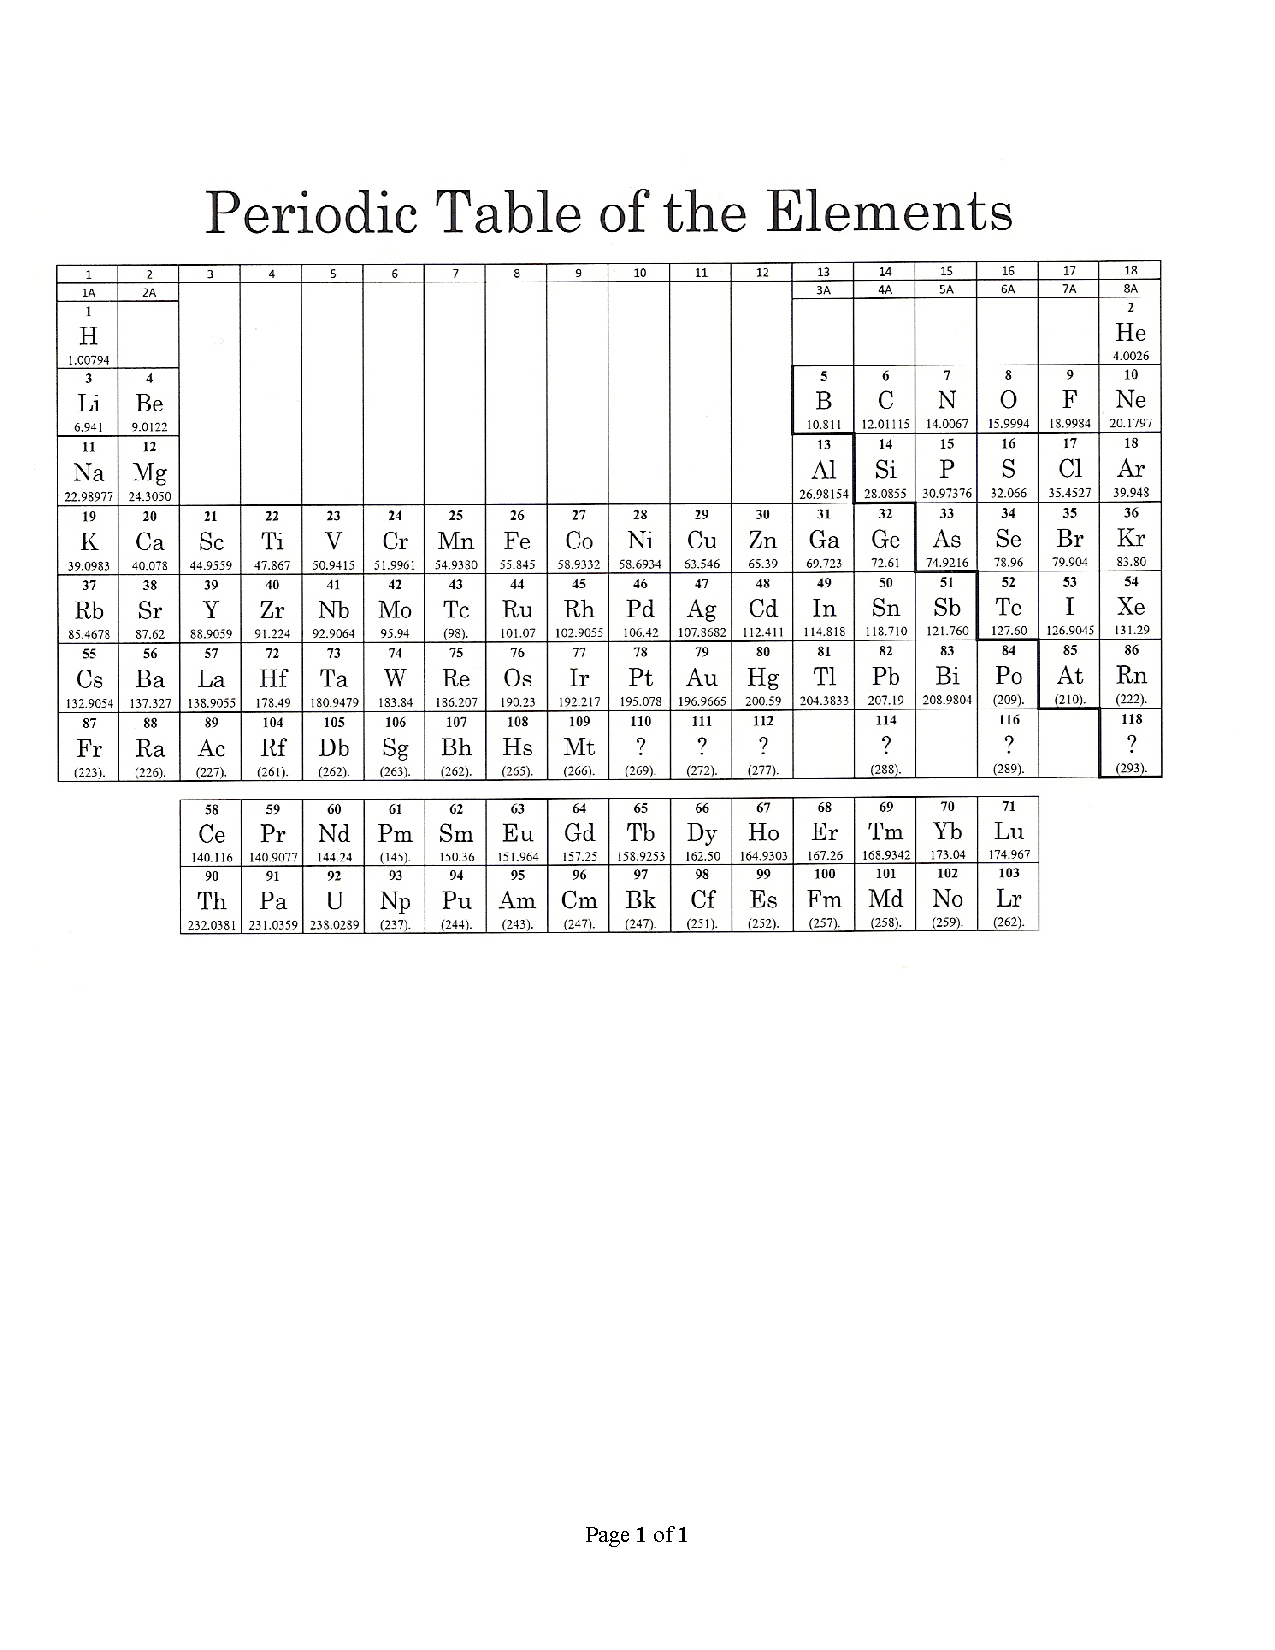
\includepdf[pages={-}]{Periodic Table for testing.pdf}

\end{document}
% END OF DOCUMENT --------------------------------------------------------------


